\chapter{Desenvolvimento} \label{cap:desenvolvimento}

\section{Hardware}

    Para a impressão dos blocos foi utilizado a impressora 3D SnapMaker com o filamento branco no material PETG. Foi impresso uma peça nas medidas definidas no capitulo 3 para testes de material e tamanho conforme apresentado na Figura \ref{figura:teste_bloco}.
    
    \begin{figure}[H]
        \caption{Teste de tamanho e material do bloco físico}
        \centering
        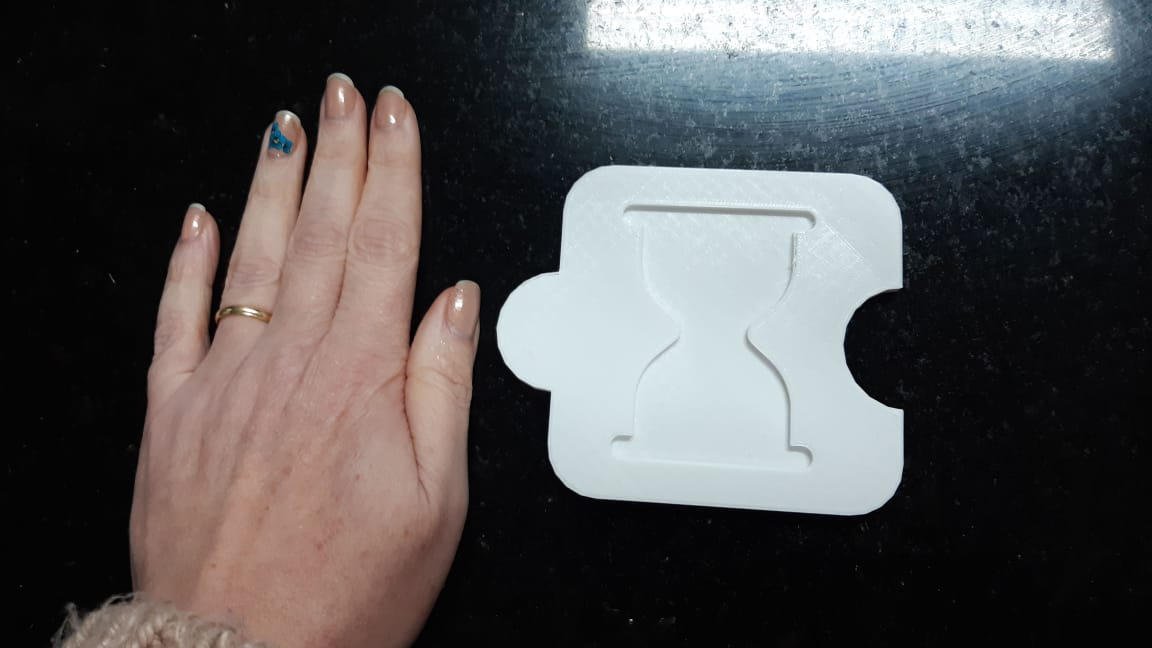
\includegraphics[width=\linewidth]{Imagens/Cap4/teste_bloco.jpeg}
        \legend{\small{Fonte: o autor (2020)}}
        \label{figura:teste_bloco}
    \end{figure}
    
    Nos testes, verificamos que o material escolhido estava dentro dos padrões aceitáveis, mantendo a peça conforme o planejado. Analisamos o tamanho da peça impressa e identificamos que estava muito grande, podendo dificultar a captura da solução pela criança. O tamanho do bloco foi reduzido para 7cm x 7cm x 5mm e um novo teste foi realizado, obtendo sucesso.
    
    Para facilitar a identificação dos blocos numéricos, alteramos o encaixe  do bloco de loop para que o bloco numérico possa encaixar lateralmente, deixando todos os blocos com encaixes laterais conforme apresentado na Figura \ref{figura:alteracao_bloco_numerico}.
    
    \begin{figure}[H]
        \caption{Alteração do bloco numérico}
        \centering
        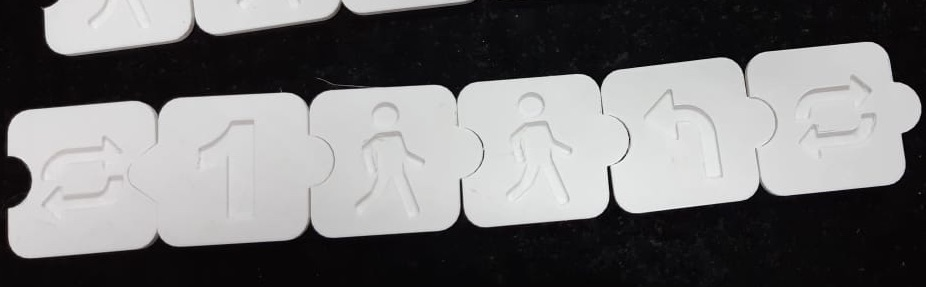
\includegraphics[width=\linewidth]{Imagens/Cap4/alteracao_bloco_numerico.jpg}
        \legend{\small{Fonte: o autor (2020)}}
        \label{figura:alteracao_bloco_numerico}
    \end{figure}
    
    As peças, impressas na cor branca, foram coloridas utilizando tinta de tecido nas cores verde, amarelo, laranja e roxo conforme apresentado na Figura \ref{figura:blocos_pintados}
    
    \begin{figure}[H]
        \caption{Alteração do bloco numérico}
        \centering
        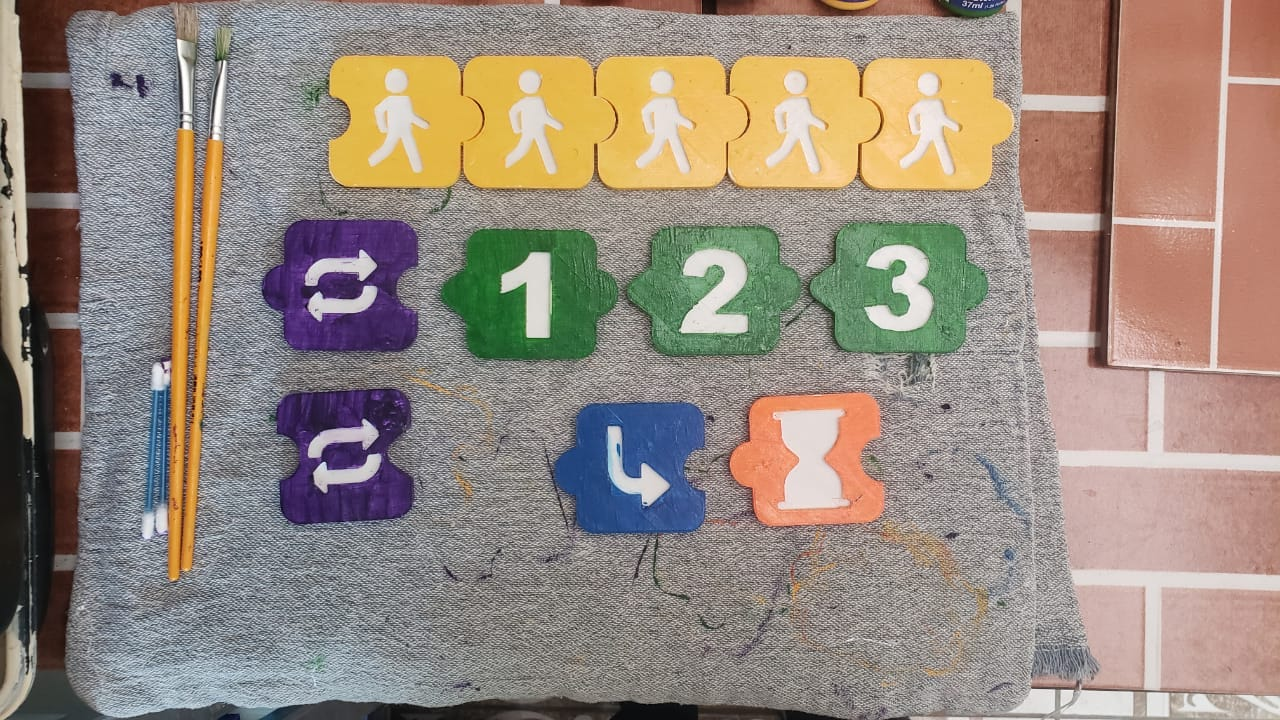
\includegraphics[width=\linewidth]{Imagens/Cap4/blocos_pintados.jpeg}
        \legend{\small{Fonte: o autor (2020)}}
        \label{figura:blocos_pintados}
    \end{figure}

\section{Software}

Para apresentar todos os softwars que compõem o aplicativo, esta seção é dividida em três subseções: software do jogo, software de reconhecimento dos blocos e por fim integração dos softwares.

    \subsection{Software do jogo}
    
    \subsection{Software de reconhecimento dos blocos}
    
    O software de reconhecimento dos blocos é uma API, isto é, uma Interface de programação de aplicações,  desenvolvida em python. Os principais módulos utilizados no desenvolvimento deste software são openCV, numpy, pytesseract, flask, json, entre outras.

    Com base no referencial teórico deste trabalho sobre visão computacional, foi desenvolvido uma API capaz de receber uma imagem dos blocos, reconhecer-los com base nas classes de blocos propostos e por fim retornar os blocos contidos na imagem submetida no formato JSON. O software de reconhecimento é limitado às seguintes restrições:
    
        \begin{itemize}
        \item Os blocos a serem reconhecidos devem exclusivamente ser desenvolvidos pelos pesquisadores e desenvolvedores deste trabalho, qualquer cópia poderá não funcionar como proposto;
        \item A imagem deve estar iluminada adequadamente (sem sombras);
        \item As cores do plano no qual os blocos estiverem dispostos devem ser diferentes das cores de qualquer um dos blocos (preferencialmente braco);
        \item A imagem deve ser capturada de forma perpendicular à superfície na qual os blocos estejam dispostos;
       \item Os blocos a serem reconhecidos devem estar centralizados na imagem e não podem estar cortados;
      \item Os blocos a serem reconhecidos não podem estar sobrepostos.
    \end{itemize}

    As etapas do desenvolvimento do algoritmo de reconhecimento dos blocos estão ilustradas no fluxograma na Figura \ref{figura:fluxo}. 
    Nas subseções subsequentes está descrito, com exemplos, o funcionamento de cada etapa do software de reconhecimento dos blocos.
    
    \begin{figure}[H]
        \caption{Fluxograma Algoritimo de Reconhecimento dos Blocos}
        \centering
        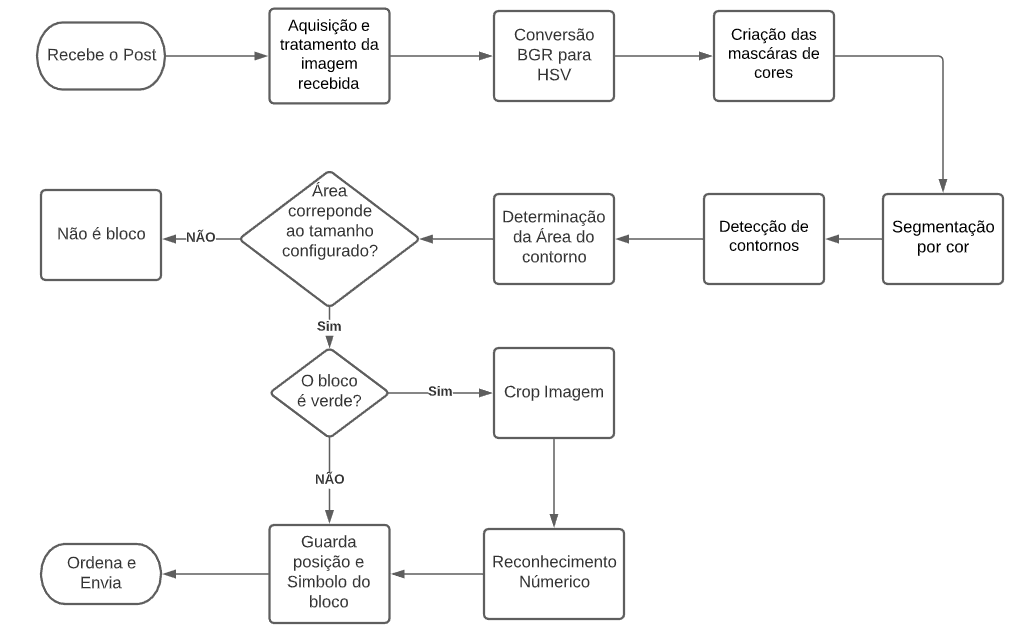
\includegraphics[width=\linewidth]{Imagens/Cap4/fluxo.PNG}
        \legend{\small{Fonte: o autor (2020)}}
        \label{figura:fluxo}
    \end{figure}


    \subsubsection{Aquisição}
    
    Após o recebimento da imagem através do protocolo http POST, é necessário converter a imagem de bytes para um vetor numpy através do comando fromstring do módulo numpy, pois é neste formato que o módulo opencv é capaz de ler as imagens. 
    
    Uma etapa comum em visão computacional é o redimensionamento  das imagens, porém neste caso não se fez necessário o redimensionamento pois as imagens já são enviadas em um tamanho pré definido pelo aplicativo jogo.

    \subsubsection{Conversão de BGR para HSV}
    O padrão HSV consiste em cor, retratado como Hue; a saturação da cor por Saturation e por fim o brilho, chamado de value, por conta disso possui o nome HSV.
    
    A etapa de conversão de BGR para HSV é fundamental, pois é por meio deste padrão que as máscaras, utilizadas para isolar cada cor da imagem é criada. Portanto é por conta desta etapa que a segmentação por cores se torna possível.

    
    \subsubsection{Segmentação Por Cor}
    Nesta etapa a imagem inicial se desfaz em N imagens, onde N  é o número de blocos distintos na imagem submetida para reconhecimento dos blocos.
    
    Nesta etapa o algoritmo compara a imagem submetida para o reconhecimento com um máscara e realiza uma filtragem de cores. Estas máscaras são criadas a partir de 3 parâmetros, o máximo de valores BGR para uma determinada cor, o mínimo valores BGR para a mesma cor, e por fim com os valores da imagem gerada através da conversão BGR para HSV da etapa anterior. 
    
    No momento em que a imagem passa por este filtro de segmentação de cor as componentes de cor que não fazem parte do espectro definido como máximo e mínimo são zeradas, resultando em uma imagem com apenas a cor que faz parte do espectro especificado, como ilustrado nas Figuras \ref{figura:ex1_original} e \ref{figura:ex1_tratado}.
    
    \begin{figure}[H]
        \caption{Exemplo de segmentação por cor - original}
        \centering
        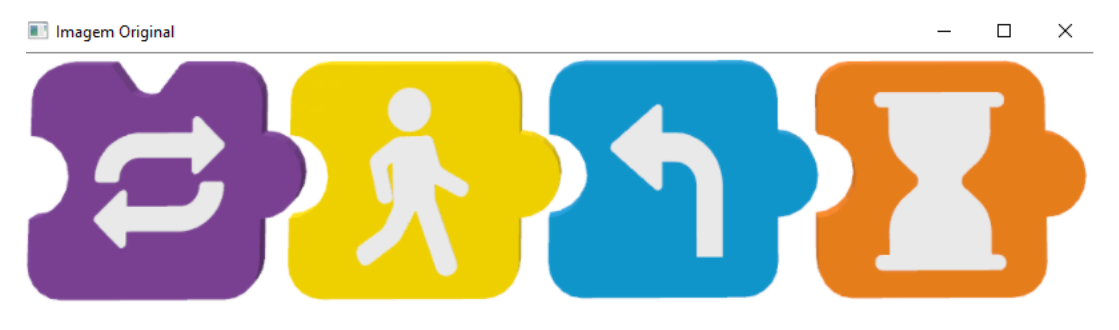
\includegraphics[width=\linewidth]{Imagens/Cap4/ex1_original.PNG}
        \legend{\small{Fonte: o autor (2020)}}
        \label{figura:ex1_original}
    \end{figure}
    
    
    \begin{figure}[H]
        \caption{Exemplo de segmentação por cor - após tratamento}
        \centering
        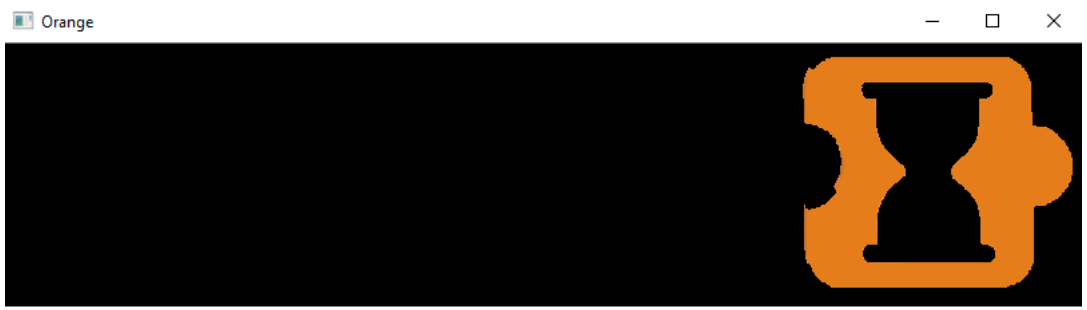
\includegraphics[width=\linewidth]{Imagens/Cap4/ex1_tratado.PNG}
        \legend{\small{Fonte: o autor (2020)}}
        \label{figura:ex1_tratado}
    \end{figure}
    
    \subsubsection{Detecção de Contorno}
    Nesta etapa, espera-se que as imagens estejam com as cores isoladas para que passem pelo processo de detecção de contorno da melhor maneira possível. Esta etapa consiste basicamente na detecção de bordas das imagens provenientes da etapa anterior.

    Através das máscaras HSV geradas, é realizada uma busca por contornos das cores que fazem parte do espectro determinado para cada cor.
    
    Depois que os contornos são encontrados, verifica-se se algum contorno possui área maior que um valor X. Se a área do contorno for maior que o valor pré determinado, o algoritmo assume, considerando a limpeza de ruídos feita na etapa de segmentação de cores e o tamanho da área encontrado nesta etapa, que aquela seção da imagem corresponde a um bloco da cor da máscara testada. Portanto por meio desta etapa, já é possível reconhecer os blocos que possuem somente uma cor para um símbolo, isto é, laranja - esperar, amarelo - caminhar, azul - virar e roxo - repetir.
    
    
    \subsubsection{Reconhecimento Numérico}
    Por fim, para o reconhecimento dos blocos numéricos se faz necessário uma etapa de OCR, ou seja, reconhecimento ótico de caracteres, pois não são possíveis descrevê-los totalmente pelas etapas anteriores, pois além da cor verde, também é preciso determinar seu símbolo.
    
    Antes da etapa de OCR, a imagem passa por um função de corte, na qual a região do símbolo a ser reconhecido é isolado com objetivo de diminuir possíveis erros da etapa de OCR. Portanto, se um bloco foi identificado como verde, obtém-se, por meio da função de achar contornos,  as coordenadas da região a ser reconhecida pela etapa de OCR e, por meio de suas coordenadas, essa região é cortada da imagem original como ilustrado nas Figuras \ref{figura:ex2_original} e \ref{figura:ex2_tratado}.
    
    \begin{figure}[H]
        \caption{Exemplo Tratametno para OCR - original}
        \centering
        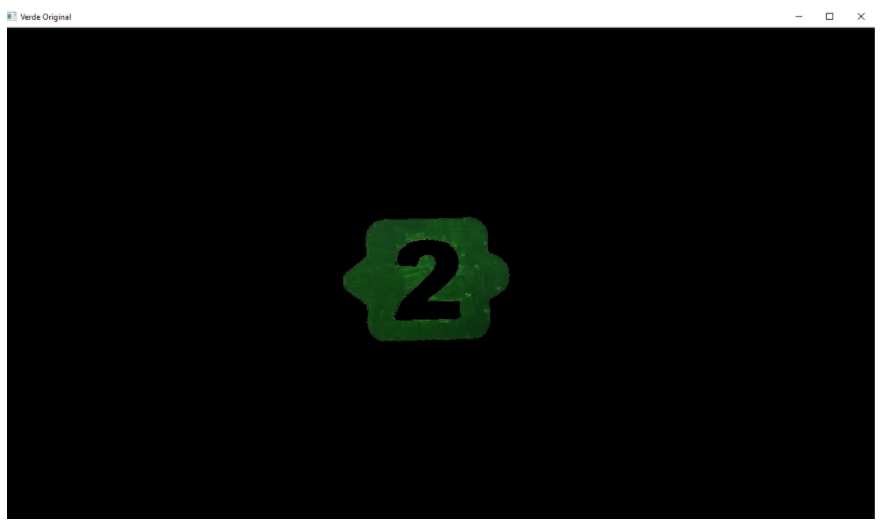
\includegraphics[width=\linewidth]{Imagens/Cap4/ex2_original.PNG}
        \legend{\small{Fonte: o autor (2020)}}
        \label{figura:ex2_original}
    \end{figure}
    
    
    \begin{figure}[H]
        \caption{Exemplo Tratametno para OCR - após tratamento}
        \centering
        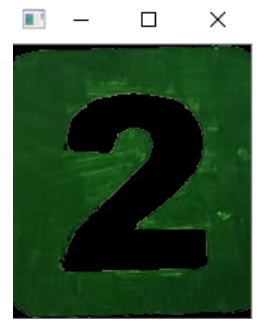
\includegraphics[width=10cm]{Imagens/Cap4/ex2_tratado.PNG}
        \legend{\small{Fonte: o autor (2020)}}
        \label{figura:ex2_tratado}
    \end{figure}
    
    Na etapa do OCR, a imagem cortada é confrontada com uma lista de 10 possíveis valores, números entre 0 e 9, e por meio do módulo de Python pytesseract e do software Tesseract, o símbolos numéricos dos blocos verdes são reconhecidos.


    \subsubsection{Envio das Informações}
    Durante as etapas anteriores, na medida em que os blocos são reconhecidos, os seus significados e, por meio da função achar contornos, suas coordenadas são armazenadas em uma estrutura de dados python conhecida com tupla.
    
    Por fim, esta estrutura que contém os blocos e suas respectivas posições na imagem é ordenada baseada nas coordenadas do menor valor de X para o maior valor de X, em outras palavras, da esquerda para a direita da imagem. Esses valores então são  encapsulados em uma estrutura JSON e são enviados como retorno da API para o aplicativo jogo.
    





    \subsection{Integração dos Softwares}
    